\section{Thursday, 18 October 2018}

\subsection{Steps}
\begin{itemize}
\item We get the columns that ends with ``MEAN'' because that columns represent the average values. In that way the dataset is more representative. After that, we work on the visualization.
\item We have done a \texttt{PCA} attempt but the \texttt{PCA} fails because we haven't deleted the version column and there are rows where the version number is not a float, it's a string like ``x.x.x'', so we eliminate the version column.
The covariance is pretty high, about $0.85$.

\begin{figure}[!htb]
\centering
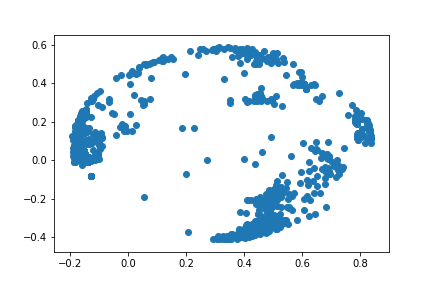
\includegraphics[width=0.5\textwidth]{../../reports/figures/PCA_AccelerometerStat.png}
\caption{Principal Component Analysis}
\label{fig:pca}
\end{figure}

\item Next, we start clustering with k-means. We analyse different groups in order to interpret the plots. We distribute the job: Ivan analyse the magnetic field, Benjamin the gyroscope and Dídimo the accelerometer.
\item If we do k-means with the complete dataset, the computer is out of memory, that is the reason why we only consider the values of 5 days.
\item We do k-means in a range of 2 to 50 clusters to know what is the ideal number of clusters. In order to get it, we use the \textit{silhouette} method and we analyse which is the best coefficient. When we already know the ideal number of clusters, we plot the graphic, showing the different groups. 

\begin{figure}[!htb]
\centering
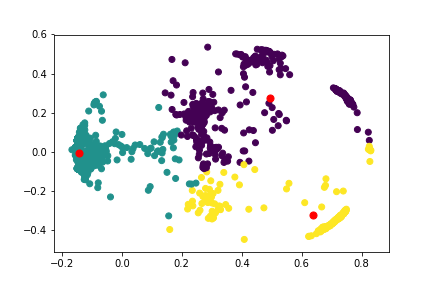
\includegraphics[width=0.5\textwidth]{../../reports/figures/KMeans_AccelerometerStat.png}
\caption{K-means clustering algorithm with best number of clusters}
\label{fig:k-means}
\end{figure}
\end{itemize}
